\documentclass[10pt]{article}
\usepackage[utf8]{inputenc}
\usepackage[T1]{fontenc}
\usepackage{graphicx}
\usepackage{tikz}
\usetikzlibrary{arrows}
\usepackage[export]{adjustbox}
\usepackage{amsmath}
\usepackage{amsfonts}
\usepackage{amssymb}
\usepackage[version=4]{mhchem}
\usepackage{stmaryrd}

\title{Problem set 11}


\author{by Maksim Al Dandan}


\begin{document}
\maketitle

\section*{Week 11. Problem set}
\begin{enumerate}
  \item Write down all possible topological sortings for the nodes of the following directed graph:
\end{enumerate}

\begin{center}
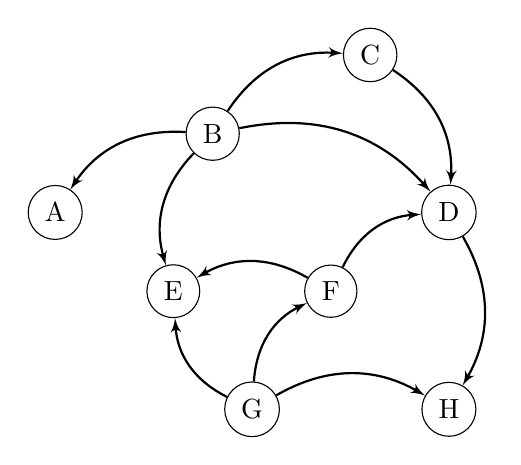
\begin{tikzpicture}

\tikzset{vertex/.style = {shape=circle,draw,minimum size=1.5em}}
\tikzset{edge/.style = {->,> = latex',thick}}
% vertices
\node[vertex] (a) at  (0,0)   {A};
\node[vertex] (b) at  (2,1)   {B};
\node[vertex] (c) at  (4,2)   {C};
\node[vertex] (d) at  (5,0)   {D};
\node[vertex] (e) at  (1.5,-1)  {E};
\node[vertex] (f) at  (3.5,-1)  {F};
\node[vertex] (g) at  (2.5,-2.5) {G};
\node[vertex] (h) at  (5,-2.5)  {H};
%edges
\draw[edge] (b) to[bend right] (a);
\draw[edge] (b) to[bend left] (c);
\draw[edge] (b) to[bend left] (d);
\draw[edge] (c) to[bend left] (d);
\draw[edge] (d) to[bend left] (h);
\draw[edge] (b) to[bend right] (e);
\draw[edge] (f) to[bend left] (d);
\draw[edge] (f) to[bend right] (e);
\draw[edge] (g) to[bend left] (e);
\draw[edge] (g) to[bend left] (f);
\draw[edge] (g) to[bend left] (h);
\end{tikzpicture}
\end{center}

\subsection*{Solution}
1. B-A-C-G-F-D-E-H \\
2. B-A-C-G-F-D-H-E \\
3. B-A-C-G-F-E-D-H \\
4. B-A-G-C-F-D-E-H \\
5. B-A-G-C-F-D-H-E \\
6. B-A-G-C-F-E-D-H \\
7. B-A-G-F-C-D-E-H \\
8. B-A-G-F-C-D-H-E \\
9. B-A-G-F-C-E-D-H \\
10. B-A-G-F-E-C-D-H \\
11. B-C-A-G-F-D-E-H \\
12. B-C-A-G-F-D-H-E \\
13. B-C-A-G-F-E-D-H \\
14. B-C-G-A-F-D-E-H \\
15. B-C-G-A-F-D-H-E \\
16. B-C-G-A-F-E-D-H \\
17. B-C-G-F-A-D-E-H \\
18. B-C-G-F-A-D-H-E \\
19. B-C-G-F-A-E-D-H \\
20. B-C-G-F-D-A-E-H \\
21. B-C-G-F-D-A-H-E \\
22. B-C-G-F-D-E-A-H \\
23. B-C-G-F-D-E-H-A \\
24. B-C-G-F-D-H-A-E \\
25. B-C-G-F-D-H-E-A \\
26. B-C-G-F-E-A-D-H \\
27. B-C-G-F-E-D-A-H \\
28. B-C-G-F-E-D-H-A \\
29. B-G-A-C-F-D-E-H \\
30. B-G-A-C-F-D-H-E \\
31. B-G-A-C-F-E-D-H \\
32. B-G-A-F-C-D-E-H \\
33. B-G-A-F-C-D-H-E \\
34. B-G-A-F-C-E-D-H \\
35. B-G-A-F-E-C-D-H \\
36. B-G-C-A-F-D-E-H \\
37. B-G-C-A-F-D-H-E \\
38. B-G-C-A-F-E-D-H \\
39. B-G-C-F-A-D-E-H \\
40. B-G-C-F-A-D-H-E \\
41. B-G-C-F-A-E-D-H \\
42. B-G-C-F-D-A-E-H \\
43. B-G-C-F-D-A-H-E \\
44. B-G-C-F-D-E-A-H \\
45. B-G-C-F-D-E-H-A \\
46. B-G-C-F-D-H-A-E \\
47. B-G-C-F-D-H-E-A \\
48. B-G-C-F-E-A-D-H \\
49. B-G-C-F-E-D-A-H \\
50. B-G-C-F-E-D-H-A \\
51. B-G-F-A-C-D-E-H \\
52. B-G-F-A-C-D-H-E \\
53. B-G-F-A-C-E-D-H \\
54. B-G-F-A-E-C-D-H \\
55. B-G-F-C-A-D-E-H \\
56. B-G-F-C-A-D-H-E \\
57. B-G-F-C-A-E-D-H \\
58. B-G-F-C-D-A-E-H \\
59. B-G-F-C-D-A-H-E \\
60. B-G-F-C-D-E-A-H \\
61. B-G-F-C-D-E-H-A \\
62. B-G-F-C-D-H-A-E \\
63. B-G-F-C-D-H-E-A \\
64. B-G-F-C-E-A-D-H \\
65. B-G-F-C-E-D-A-H \\
66. B-G-F-C-E-D-H-A \\
67. B-G-F-E-A-C-D-H \\
68. B-G-F-E-C-A-D-H \\
69. B-G-F-E-C-D-A-H \\
70. B-G-F-E-C-D-H-A \\
71. G-B-A-C-F-D-E-H \\
72. G-B-A-C-F-D-H-E \\
73. G-B-A-C-F-E-D-H \\
74. G-B-A-F-C-D-E-H \\
75. G-B-A-F-C-D-H-E \\
76. G-B-A-F-C-E-D-H \\
77. G-B-A-F-E-C-D-H \\
78. G-B-C-A-F-D-E-H \\
79. G-B-C-A-F-D-H-E \\
80. G-B-C-A-F-E-D-H \\
81. G-B-C-F-A-D-E-H \\
82. G-B-C-F-A-D-H-E \\
83. G-B-C-F-A-E-D-H \\
84. G-B-C-F-D-A-E-H \\
85. G-B-C-F-D-A-H-E \\
86. G-B-C-F-D-E-A-H \\
87. G-B-C-F-D-E-H-A \\
88. G-B-C-F-D-H-A-E \\
89. G-B-C-F-D-H-E-A \\
90. G-B-C-F-E-A-D-H \\
91. G-B-C-F-E-D-A-H \\
92. G-B-C-F-E-D-H-A \\
93. G-B-F-A-C-D-E-H \\
94. G-B-F-A-C-D-H-E \\
95. G-B-F-A-C-E-D-H \\
96. G-B-F-A-E-C-D-H \\
97. G-B-F-C-A-D-E-H \\
98. G-B-F-C-A-D-H-E \\
99. G-B-F-C-A-E-D-H \\
100. G-B-F-C-D-A-E-H \\
101. G-B-F-C-D-A-H-E \\
102. G-B-F-C-D-E-A-H \\
103. G-B-F-C-D-E-H-A \\
104. G-B-F-C-D-H-A-E \\
105. G-B-F-C-D-H-E-A \\
106. G-B-F-C-E-A-D-H \\
107. G-B-F-C-E-D-A-H \\
108. G-B-F-C-E-D-H-A \\
109. G-B-F-E-A-C-D-H \\
110. G-B-F-E-C-A-D-H \\
111. G-B-F-E-C-D-A-H \\
112. G-B-F-E-C-D-H-A \\
113. G-F-B-A-C-D-E-H \\
114. G-F-B-A-C-D-H-E \\
115. G-F-B-A-C-E-D-H \\
116. G-F-B-A-E-C-D-H \\
117. G-F-B-C-A-D-E-H \\
118. G-F-B-C-A-D-H-E \\
119. G-F-B-C-A-E-D-H \\
120. G-F-B-C-D-A-E-H \\
121. G-F-B-C-D-A-H-E \\
122. G-F-B-C-D-E-A-H \\
123. G-F-B-C-D-E-H-A \\
124. G-F-B-C-D-H-A-E \\
125. G-F-B-C-D-H-E-A \\
126. G-F-B-C-E-A-D-H \\
127. G-F-B-C-E-D-A-H \\
128. G-F-B-C-E-D-H-A \\
129. G-F-B-E-A-C-D-H \\
130. G-F-B-E-C-A-D-H \\
131. G-F-B-E-C-D-A-H \\
132. G-F-B-E-C-D-H-A \\

\begin{enumerate}
  \setcounter{enumi}{1}
  \item Give an example of a directed graph $G=(V, E)$, a source vertex $s$, and a set of edges $T \subseteq E$ such that
\end{enumerate}

\begin{itemize}
  \item $T$ forms a tree and
  \item for each vertex $v \in V$, the unique simple path in the graph $(V, T)$ from $s$ to $v$ is a shortest path in $G$, yet
  \item the set of edges $T$ cannot be produced by running BFS on $G$, no matter how the vertices are ordered in the adjacency lists.
\end{itemize}

\subsection*{Solution}
Consider the following directed graph $G=(V, E)$, where $V = \{s, a, b, c\}$ and $E = \{(s, a), (s, b), (a, c), (b, c)\}$.

\begin{center}
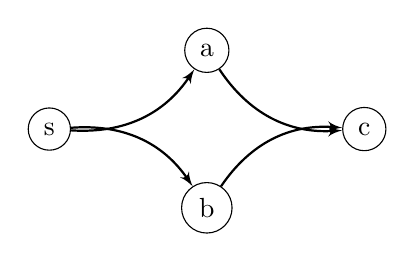
\begin{tikzpicture}
\tikzset{vertex/.style = {shape=circle,draw,minimum size=1.5em}}
\tikzset{edge/.style = {->,> = latex',thick}}
% vertices
\node[vertex] (s) at  (0,0)   {s};
\node[vertex] (a) at  (2,1)   {a};
\node[vertex] (b) at  (2,-1)  {b};
\node[vertex] (c) at  (4,0)   {c};
%edges
\draw[edge] (s) to[bend right] (a);
\draw[edge] (s) to[bend left] (b);
\draw[edge] (a) to[bend right] (c);
\draw[edge] (b) to[bend left] (c);
\end{tikzpicture}
\end{center}

The source vertex is $s$. The set of edges $T = \{(s, a), (a, c)\}$ forms a tree. For each vertex $v \in V$, the unique simple path in the graph $(V, T)$ from $s$ to $v$ is a shortest path in $G$. However, the set of edges $T$ cannot be produced by running BFS on $G$, no matter how the vertices are ordered in the adjacency lists. This is because BFS would always include the edge $(s, b)$ in $T$ before it includes $(a, c)$, since $b$ is a direct neighbor of $s$ and $c$ is not.

\end{document}